\documentclass[]{IEEEtran}

\usepackage[utf8]{inputenc}
\usepackage{float, graphicx, booktabs, siunitx}
\usepackage{microtype, amsmath, minted}

\usepackage{inconsolata}
\usepackage[italian]{babel}

\newcommand{\url}[1]{\mintinline{text}{#1}}
\newcommand{\code}[1]{\mintinline{C++}{#1}}
\newcommand{\module}[1]{\textsf{\small #1}}

\title{Sessione hands-on del tutorial {\huge ``Exploiting Automatic Abstraction and the FMI Standard to build Cycle-accurate Virtual Platforms from Heterogeneous IPs"}}
\author{Massimiliano Incudini - VR433300}

\begin{document}
\maketitle

\begin{abstract}
    Il seguente documento documenta il lavoro svolto durante la seconda parte del modulo di laboratorio del corso Progettazione di Sistemi Embedded (aa 2018/2019). Il suo obiettivo è illustrare passo per passo la procedura che genera i pacchetti \code{fmu} a partire da sorgenti eterogenei forniti e simulare il comportamento dell'intero sistema fatto dalla connessione di questi componenti.
\end{abstract}

\section{Introduzione}

Il progetto consiste nel modificare, compilare e interconnettere gli elementi del sistema in Figura~\ref{fig:system} esportati secondo il formato del protocollo \emph{Functional Mockup Interface}. 

\begin{figure}[htbp]
    \centering
    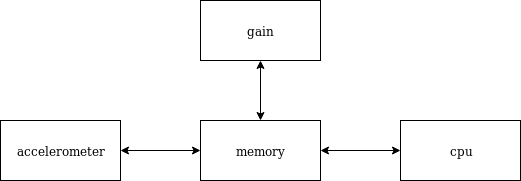
\includegraphics[width=0.45\textwidth]{fmi_schemi/system.png}
    \caption{Sistema}
    \label{fig:system}
\end{figure}

\begin{figure*}[h]
    \centering
    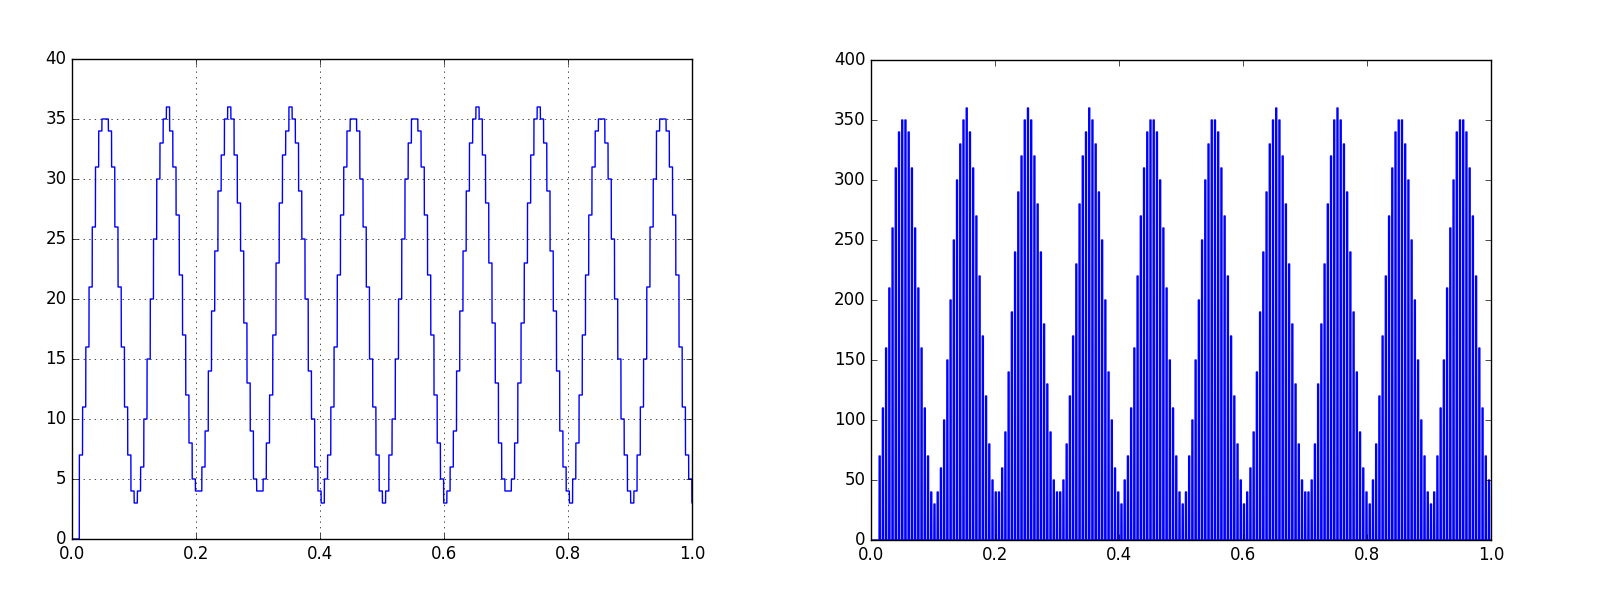
\includegraphics[width=0.9\textwidth]{fmi_schemi/images.png}
    \caption{Risultato della simulazione con PyFMI. A sinistra il segnale in input al gain, a destra l'output.}
    \label{fig:fmioutput}
\end{figure*}

Le componenti del sistema comunicano tramite memory-mapping. 

\section{Protocollo FMI}

FMI è uno standard indipendente pensato per supportare sia \emph{scambio di modelli} che \emph{cosimulazione} di modelli dinamici attraverso una combinazione di file XML e codice C (sia compilato che in formato sorgente)\cite{fmi}.

Lo standard, tra le altre cose, definisce:
\begin{itemize}
    \item una API (C) per eseguire le funzioni di una FMU attraverso codice C;
    \item l'FMI Description Schema, file XML-Schema che descrive come deve essere il documento contenente le informazioni statiche (di interfaccia) della FMU; queste informazioni sono contenute in un file \code{modelDescription.xml}.
\end{itemize}

\section{Modulo \module{Gain}}

Questa sezione si riferisce al contenuto della directory \url{/fmi_lesson/models/gain}.

Il modulo \module{Gain} è descritto nel linguaggio C++ all'interno della sottodirectory \url{/cpp}. La sua interfaccia viene modificata aggiungendo un campo \code{result} di tipo \code{int}. All'interno del codice, questa variabile implementa la funzione
\[ \code{result} = \begin{cases} \code{data} * 10, & \code{data_rdy} = 1 \\ 0 & \text{altrimenti} \end{cases} \]
Una volta che il dato è stato scritto poniamo \code{result_rdy} alto. Tale flag verrà ri-settato basso in altri punti di codice. 

Una volta processato con \code{cmake} e \code{make} otteniamo un eseguibile binario \code{.so}. All'interno di \url{/fmu} è presente il file XML di descrizione della piattaforma che deve essere anch'esso modificato. All'interno viene aggiunta la porta definita nei sorgenti:
\begin{minted}{xml}
<ScalarVariable 
    causality="output" 
    description="result data port" 
    name="result" 
    valueReference="1" 
    variability="discrete">
    
        <Integer start="0"/>
</ScalarVariable>
\end{minted}
Come possiamo vedere la variabile è di output, di tipo intero ed il suo identificatore è settato ad $1$. Ogni variabile è difatti identificata dalla coppia $\langle \code{tipo}, n \rangle$. Essendoci già una variabile intera (campo \code{data} in input) non utilizziamo il primo numero identificativo per il tipo ($0$) ma il suo successore. 
Attraverso il comando \code{make} viene preso il file \code{.so} generato dalla compilazione del modello, ed impacchettato insieme al documento XML per generare la \emph{functional mockup unit} (file \code{.fmu}). 

\section{Moduli da compilare}

Questa sezione si riferisce al contenuto della directory \url{/fmi_lesson/models/[nome modello]}.

I moduli del progetto presenti unicamente come sorgenti che devono essere compilati sono:
\begin{itemize}
    \item \module{accelerometer}: sensore analogico descritto in Verilog-A;
    \item \module{m6502}: processore descritto in Verilog;
    \item \module{mem}: memoria scritta in Verilog.
\end{itemize}
Ognuno di questi progetti viene elaborato in un pacchetto \code{fmu} attraverso le utility del software HIFSuite.
\begin{enumerate}
    \item Il primo step consiste nell'avviare il frontend \code{verilog2hif}, che a partire dal Verilog restituisce lo stesso file secondo la rappresentazione interna del tool;
    \item il secondo step consiste nell'applicare delle ottimizzazioni;
    \item il terzo step consiste nell'avviare il backend \code{hif2sc} che restituisce la rappresentazione del modulo in C++;
    \item il quarto step consiste nell'avviare l'utility \code{hif2vp} che restutisce il documento XML relativo alla rappresentazione del modulo;
    \item il quinto step consiste nel compilare il codice C++ e comprimerlo in un archivio \code{zip} insieme al documento XML.
\end{enumerate}

\section{Simulazione del sistema}

Questa sezione si riferisce al contenuto della directory \url{/fmi_lesson/coordinator}.

Per simulare il sistema viene utilizzato il framework PyFMI basato su linguaggio Python. I comandi necessari per la simulazione sono presenti nel file \url{coordinator.py}. I moduli, ad esempio il \module{Gain}, vengono caricati come segue:
\begin{minted}{python}
# Carico le FMU
gain = load_fmu('./fmus/gain.fmu')
# Inizializzo le FMU
gain.initialize()
# Eseguo uno step di computazione
gain.do_step( ... )
# Leggo le porte di output
gain.get_integer(GAIN_RESULT)
# La scrittura delle porte invece è
# tutta nel metodo data_exchange
\end{minted}

Possiamo vedere in Figura~\ref{fig:fmioutput}. Nella parte a sinistra abbiamo il segnale in input al \module{gain}. A destra abbiamo il segnale. Come possiamo vedere i valori sono moltiplicati $\times 10$ rispetto all'input, meno che alcuni punti: questi sono gli istanti nei quali \code{data_rdy}. 

\bibliographystyle{IEEEtran}
\bibliography{biblio}

\end{document}
